Since the SphericalTNBBeta distribution does not require rejection sampling, it admits significantly
faster sampling than the vMF distribution:
\begin{figure}[H]
    \centering
    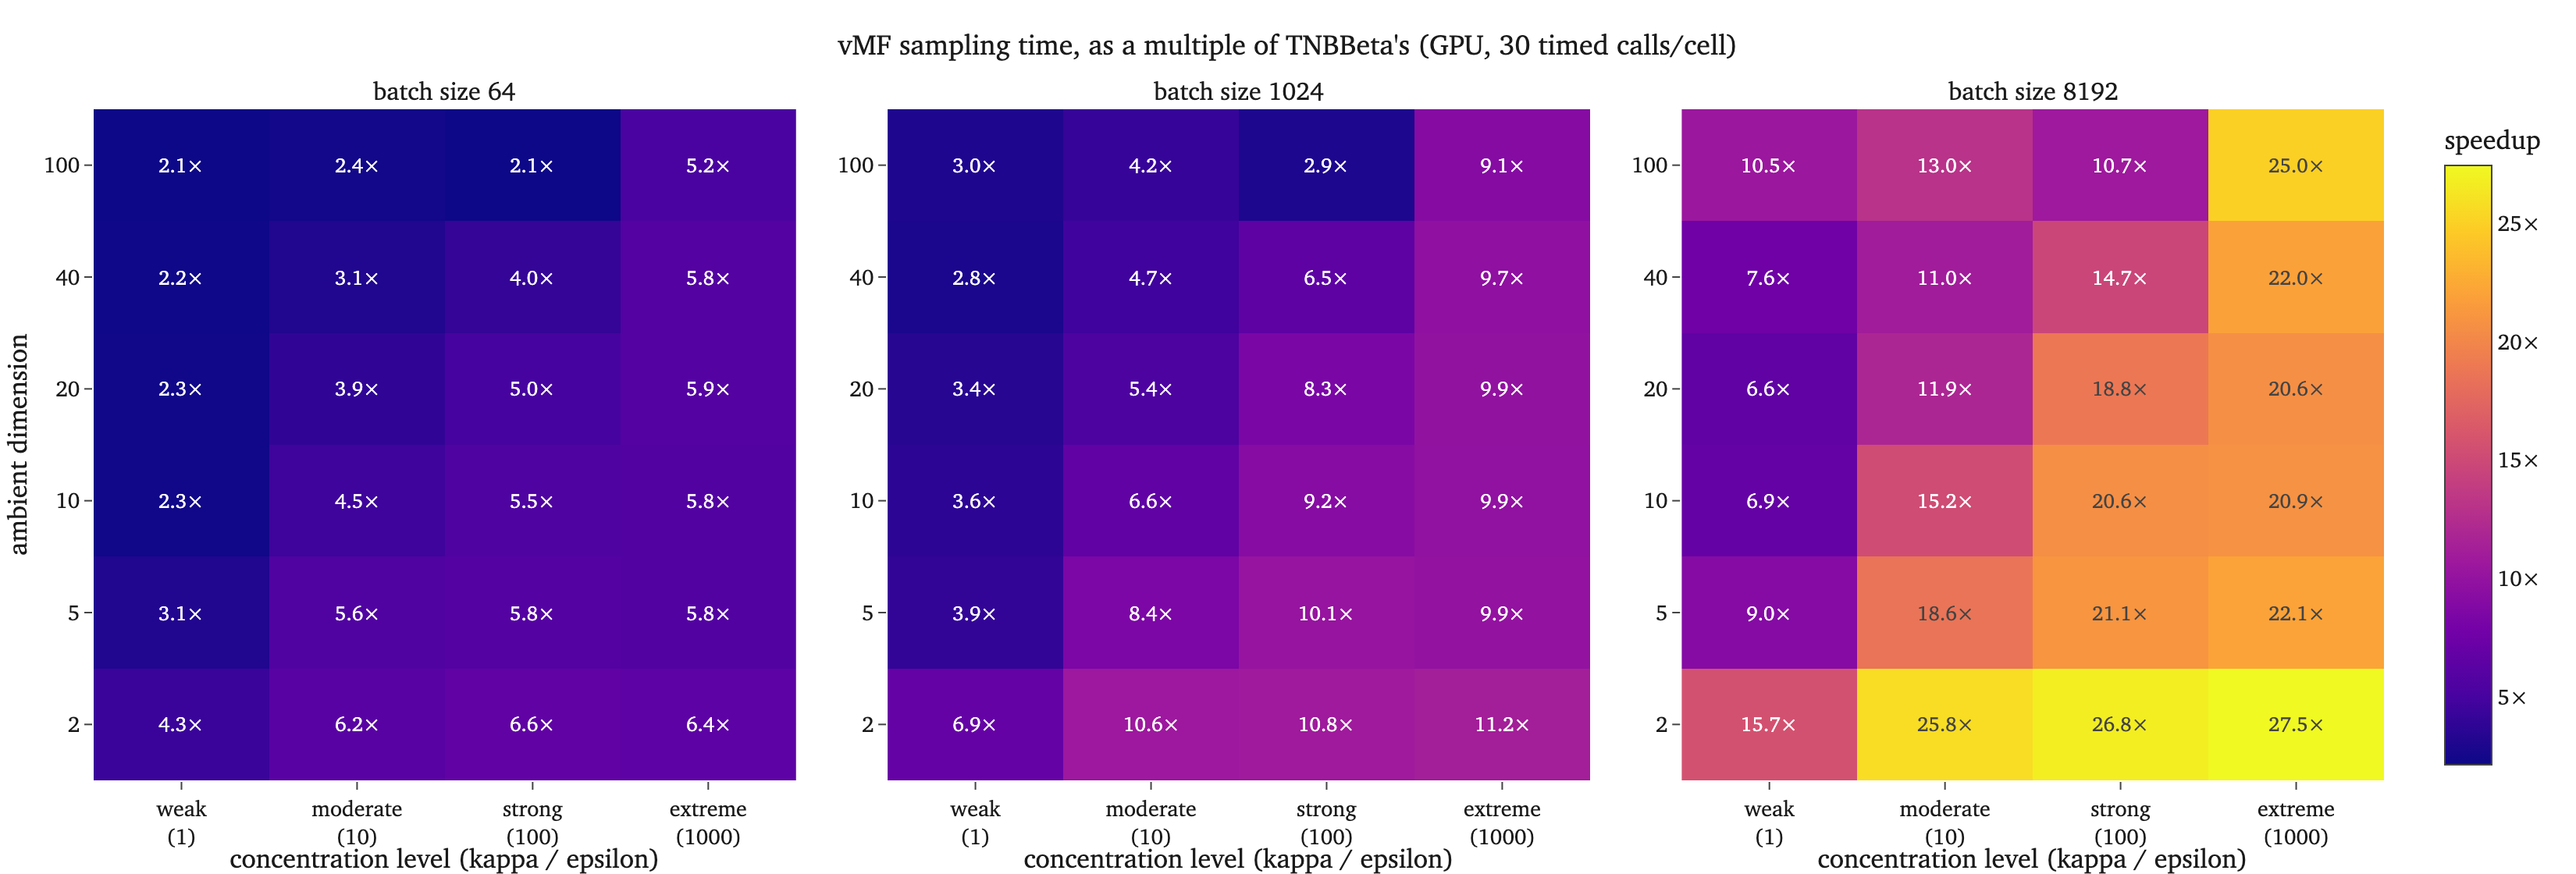
\includegraphics[width=\textwidth]{assets/sampling_speed_heatmap.png}
    \caption{Comparison between sampling time for a single SphericalTNBBeta batch and a single vMF batch on one GPU}
\end{figure}
At the $d=64$ level it is worth noting that this speedup is comparable to that of the power-spherical distribution,
as outlined in Figure 2b of \cite{decao2020powersphericaldistribution}. Given more recent deep generative
models tend to employ larger batch sizes on the order of $10^3$, we additionally included results for higher batch sizes
and note that the speedup is even more pronounced in those cases.

Sampling speed aside, we find that TNBBeta-VAE performance is nearly identical that of the power spherical VAE and the S-VAE, using
binarized MNIST \citep{lecun1998mnist} as a simple example.
\begin{figure}[H]
    \centering
    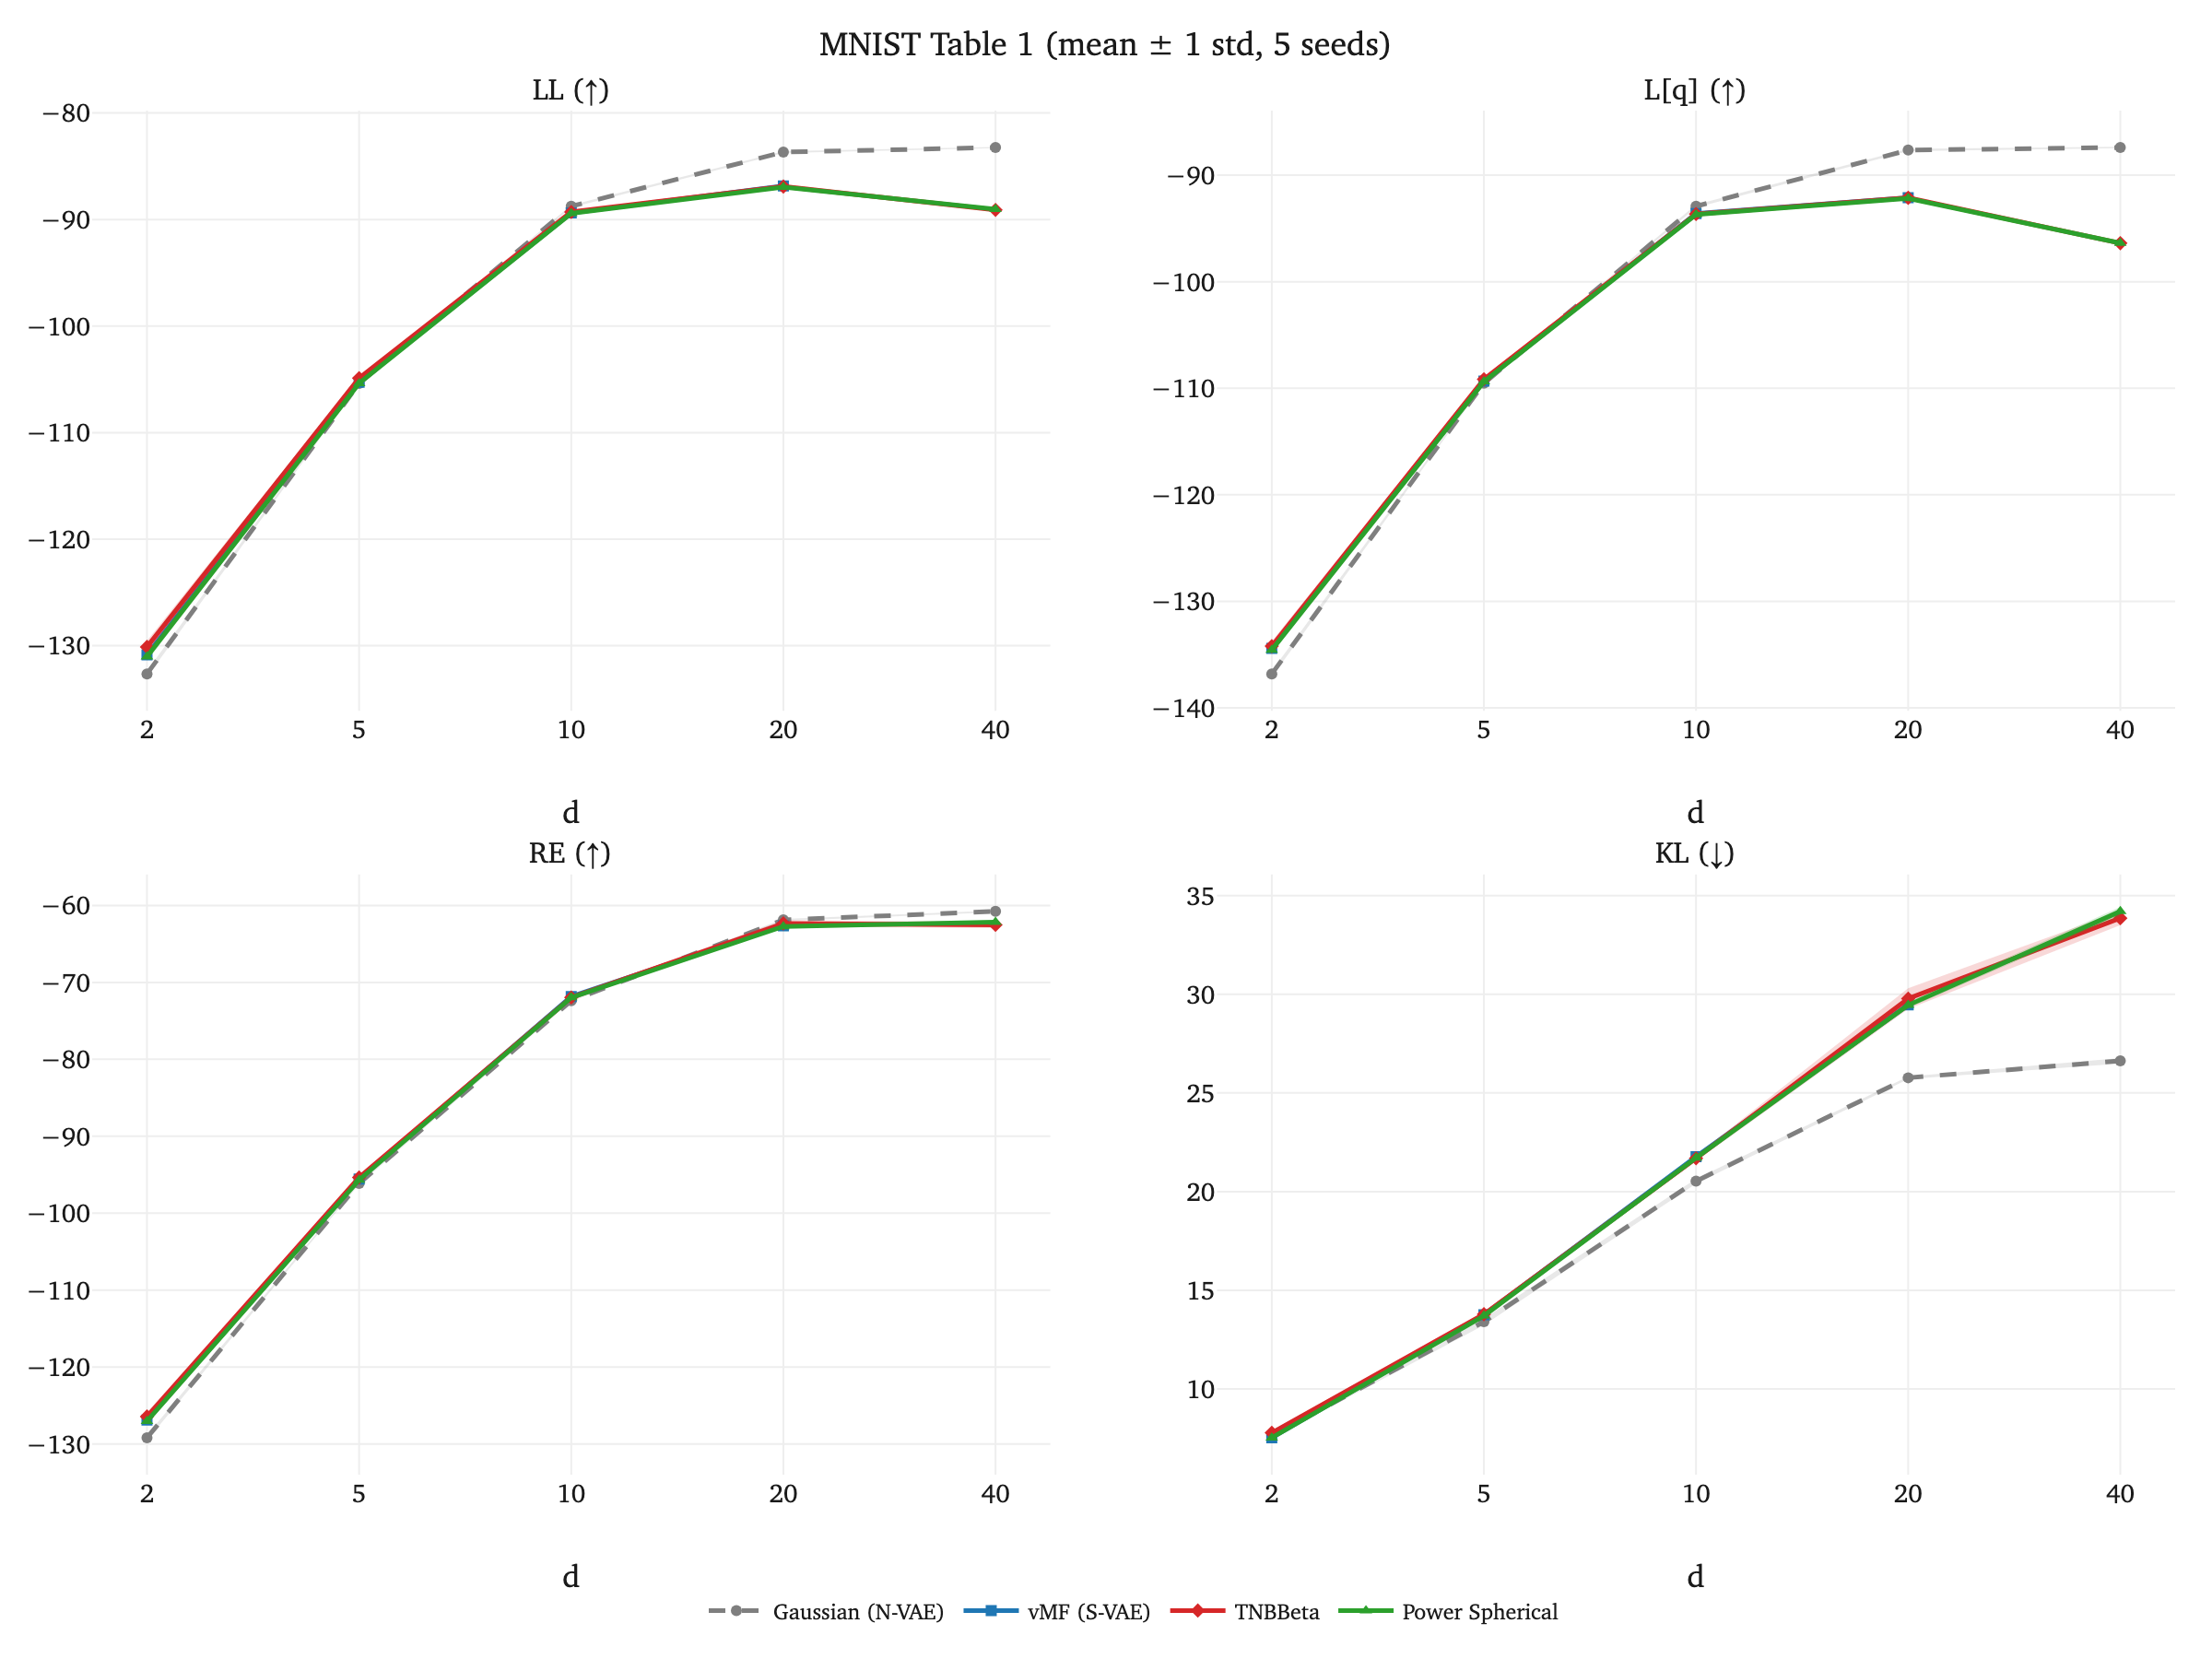
\includegraphics[width=\textwidth * 6 / 8]{assets/mnist_table1_lines.png}
    \caption{MNIST reconstruction quality, mean $\pm 1$ standard deviation over 5 seeds}
    \label{fig:mnist-table1-lines}
\end{figure}
The above result is rather unsurprising once we consider the structure of the latent space for the S-VAE and TNBBeta-VAE.
\begin{figure}[H]
    \centering
    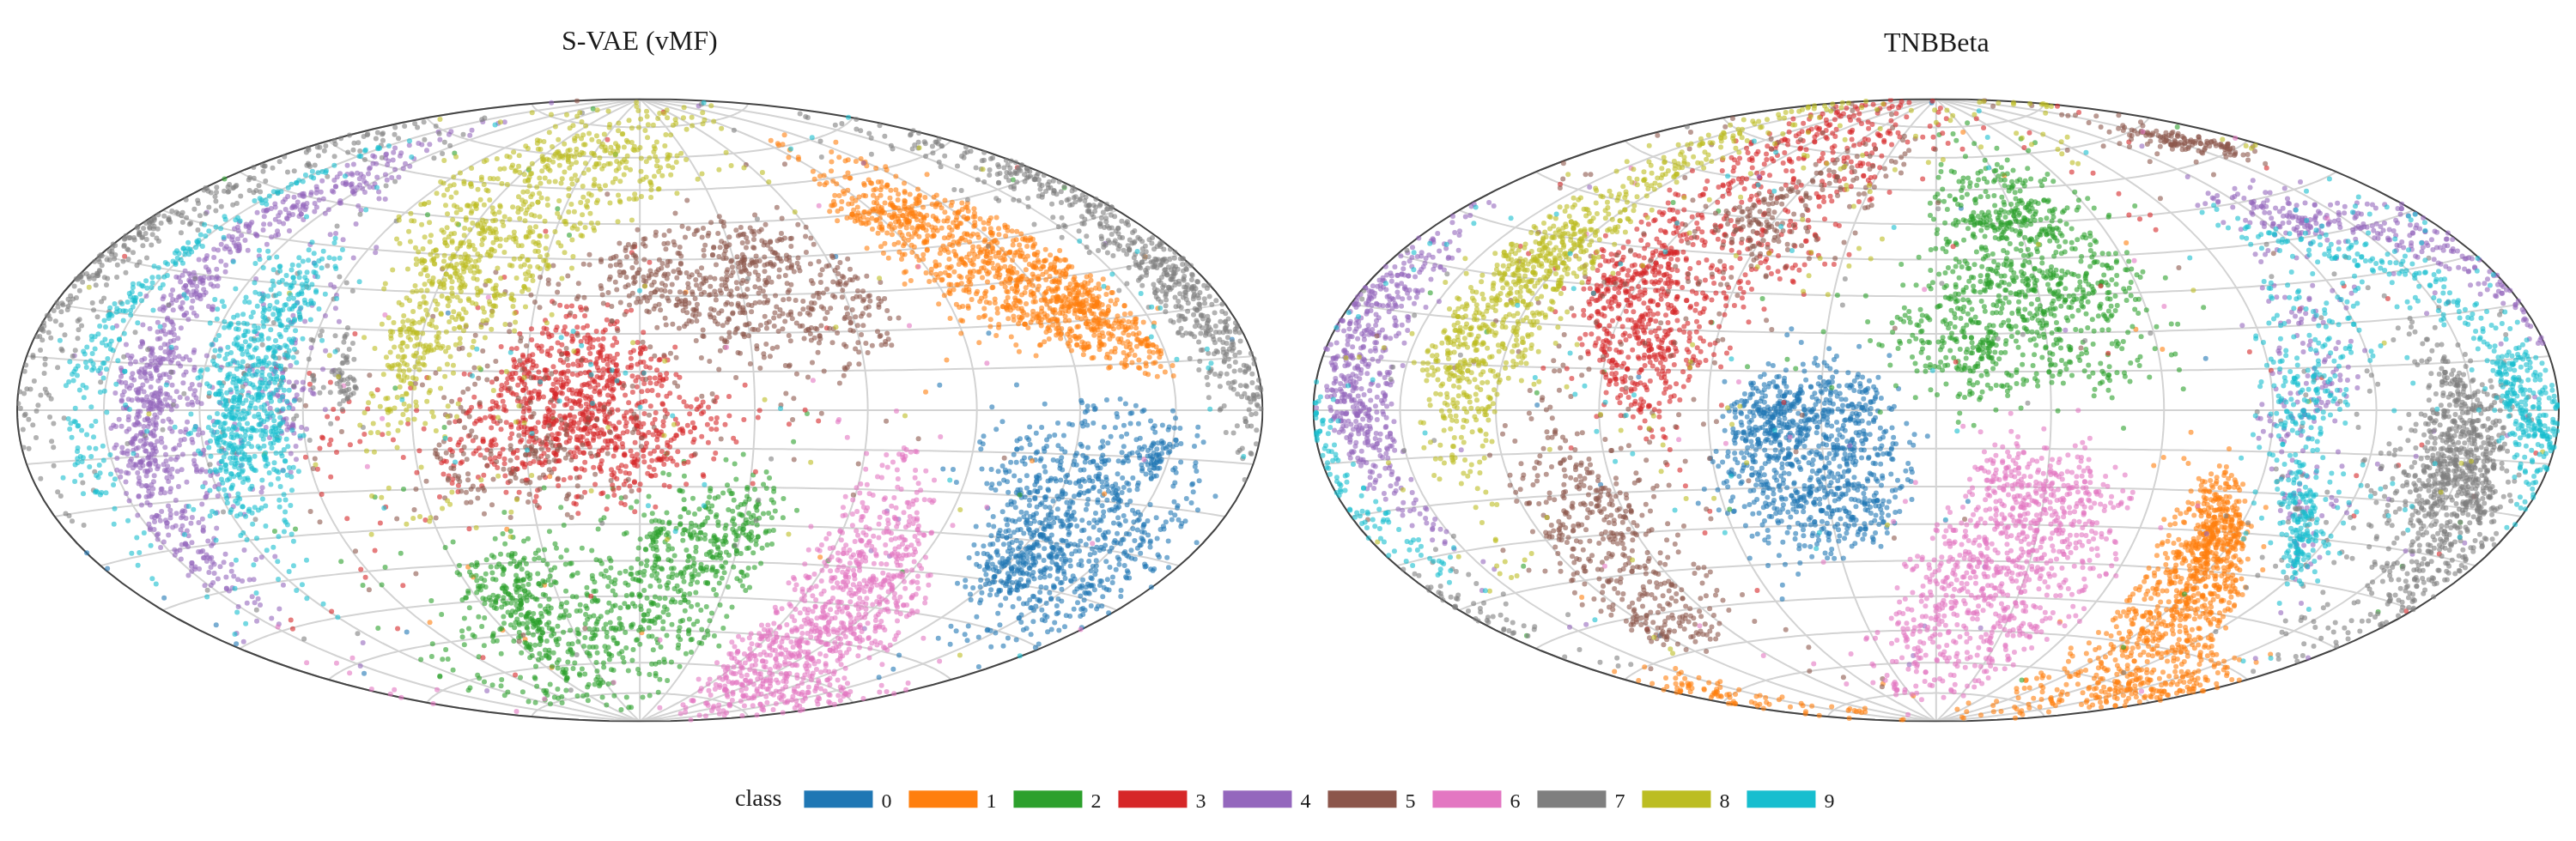
\includegraphics[width=\textwidth]{assets/hammer_mnist_vmfs_d2_seed0_vs_mnist_tnbs_d2_seed0.png}
    \caption{Hammer projection of MNIST embeddings in $\mathbb{S}^2$}
    \label{fig:hammer}
\end{figure}
\Cref{fig:hammer} illustrates that the vMF and TNBBeta latent spaces both form cap-like structures around the unit hypersphere
in low dimensions, and \Cref{thm:limiting-tnbbeta} shows that, as $p \to 1$, this similarity in shape holds for higher
dimensions. \Cref{fig:appx-posterior-traj} shows that this asymptotic limit is indeed reached during training for various
latent dimensions.

One is then left to wonder where these posteriors diverge in shape. Variational graph autoencoders (VGAEs) \citep{kipf2016variationalgraphautoencoders}
provide one avenue to explore such differences. We trained a series of VGAEs on citation networks,
namely Cora, Pubmed, Citeseer \cite{https://doi.org/10.1609/aimag.v29i3.2157}, and computer science
coauthorship networks from the Microsoft Academic Graph, as constructed in \cite{shchur2019overlappingcommunitydetectiongraph}. For each dataset
and posterior approximation, we trained two VGAEs: one using the training adjacency matrix and individual node features, and one without
individual node features. After training, we evaluated link prediction AUC and AP on a held-out set of edges.
\Cref{fig:features-onoff-bars} shows that link prediction performance is indistinguishable between all posterior families
with node features, while Gaussian and SphericalTNBBeta posteriors dominate without node features.
\begin{figure}[H]
    \centering
    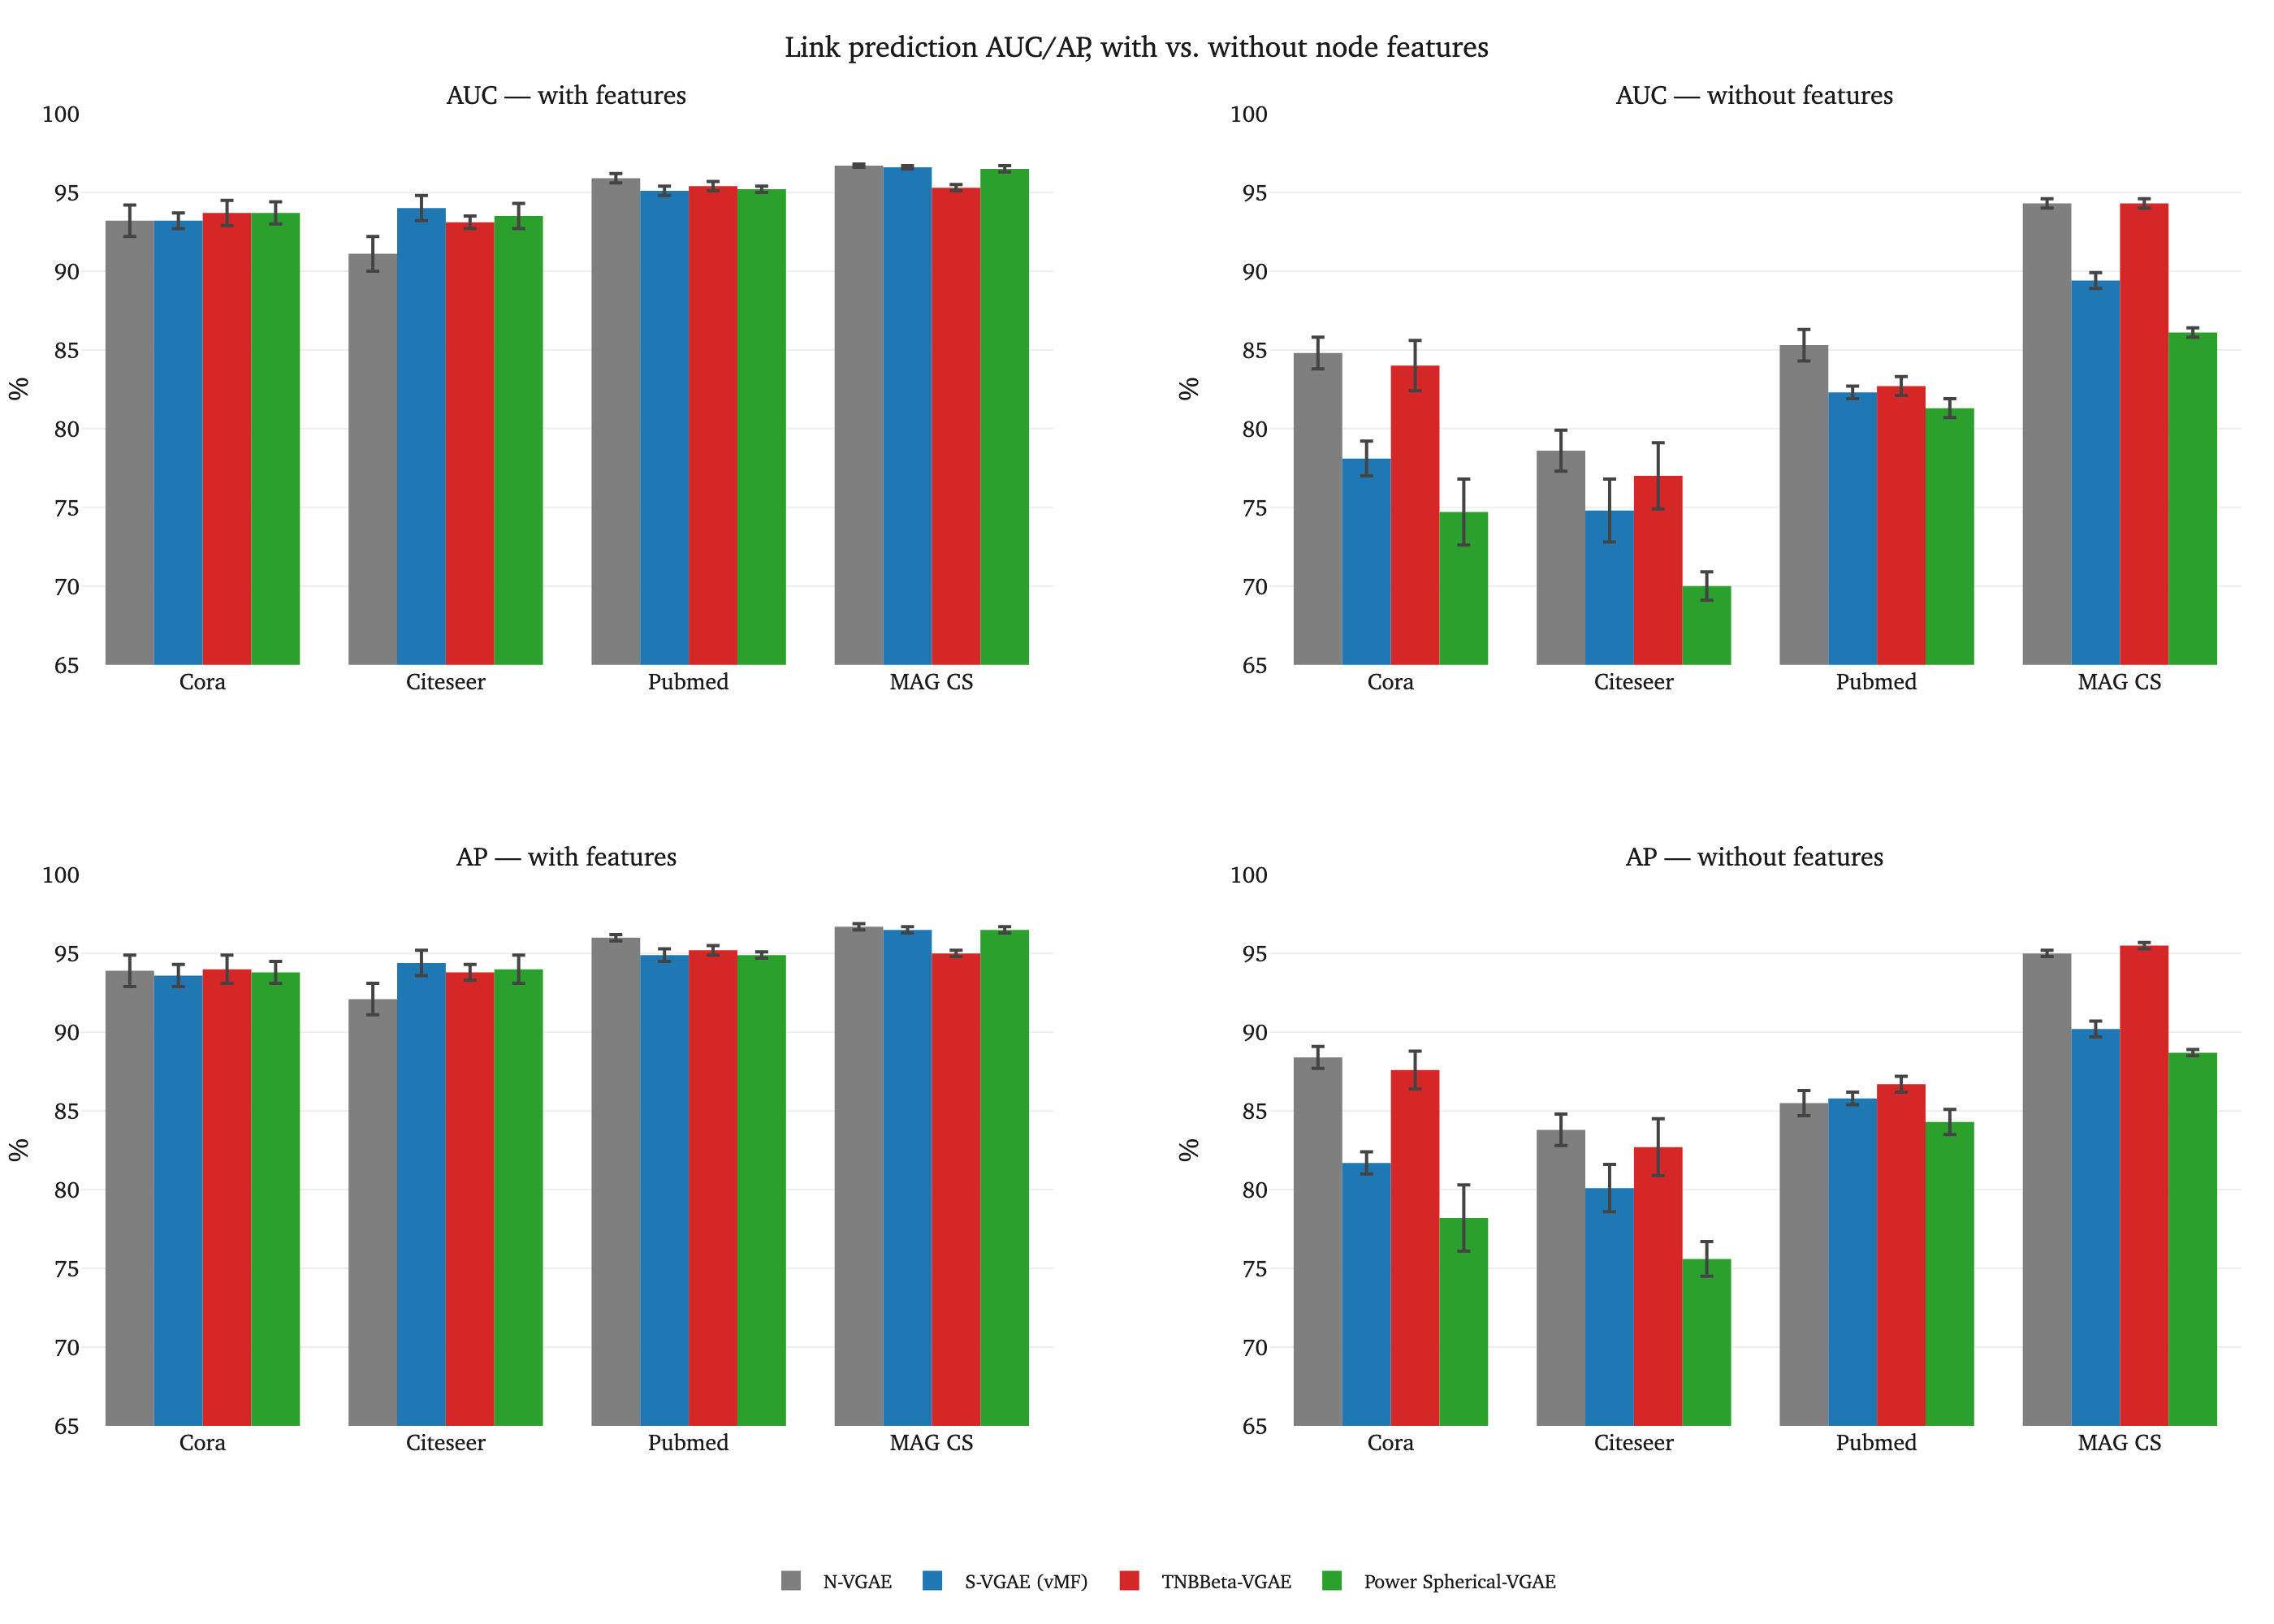
\includegraphics[width=\textwidth]{assets/features_onoff_bars.png}
    \caption{Link-prediction AUC (top) and AP (bottom), with features (left) vs.\ without (right), mean
    $\pm 1$ standard deviation over 5 seeds}
    \label{fig:features-onoff-bars}
\end{figure}

\Cref{fig:appx-posterior-traj} in appendix B shows that, in the MNIST experiments, the posterior $\varepsilon$ parameter always landed
in a unimodal regime (see \Cref{thm:modality-tnbbeta}). Let $m$ denote that threshold. In the above graph representation experiments,
we found $m$ to be consistently within a \textit{bimodal} regime. To understand what node characteristics affect the modality of
the per-point posterior, we constructed a series of synthetic graphs. Each graph contains ten communities, with 50 nodes per community.
We assign each graph a probability $p_{\text{out}}$, and construct the adjacency matrix $A_{ij} \sim \text{Bernoulli}(p_{\text{out}})$
if nodes $i$ and $j$ do not share a community. Otherwise, we draw $A_{ij} \sim \text{Bernoulli}(0.3)$.
\begin{figure}[H]
    \centering
    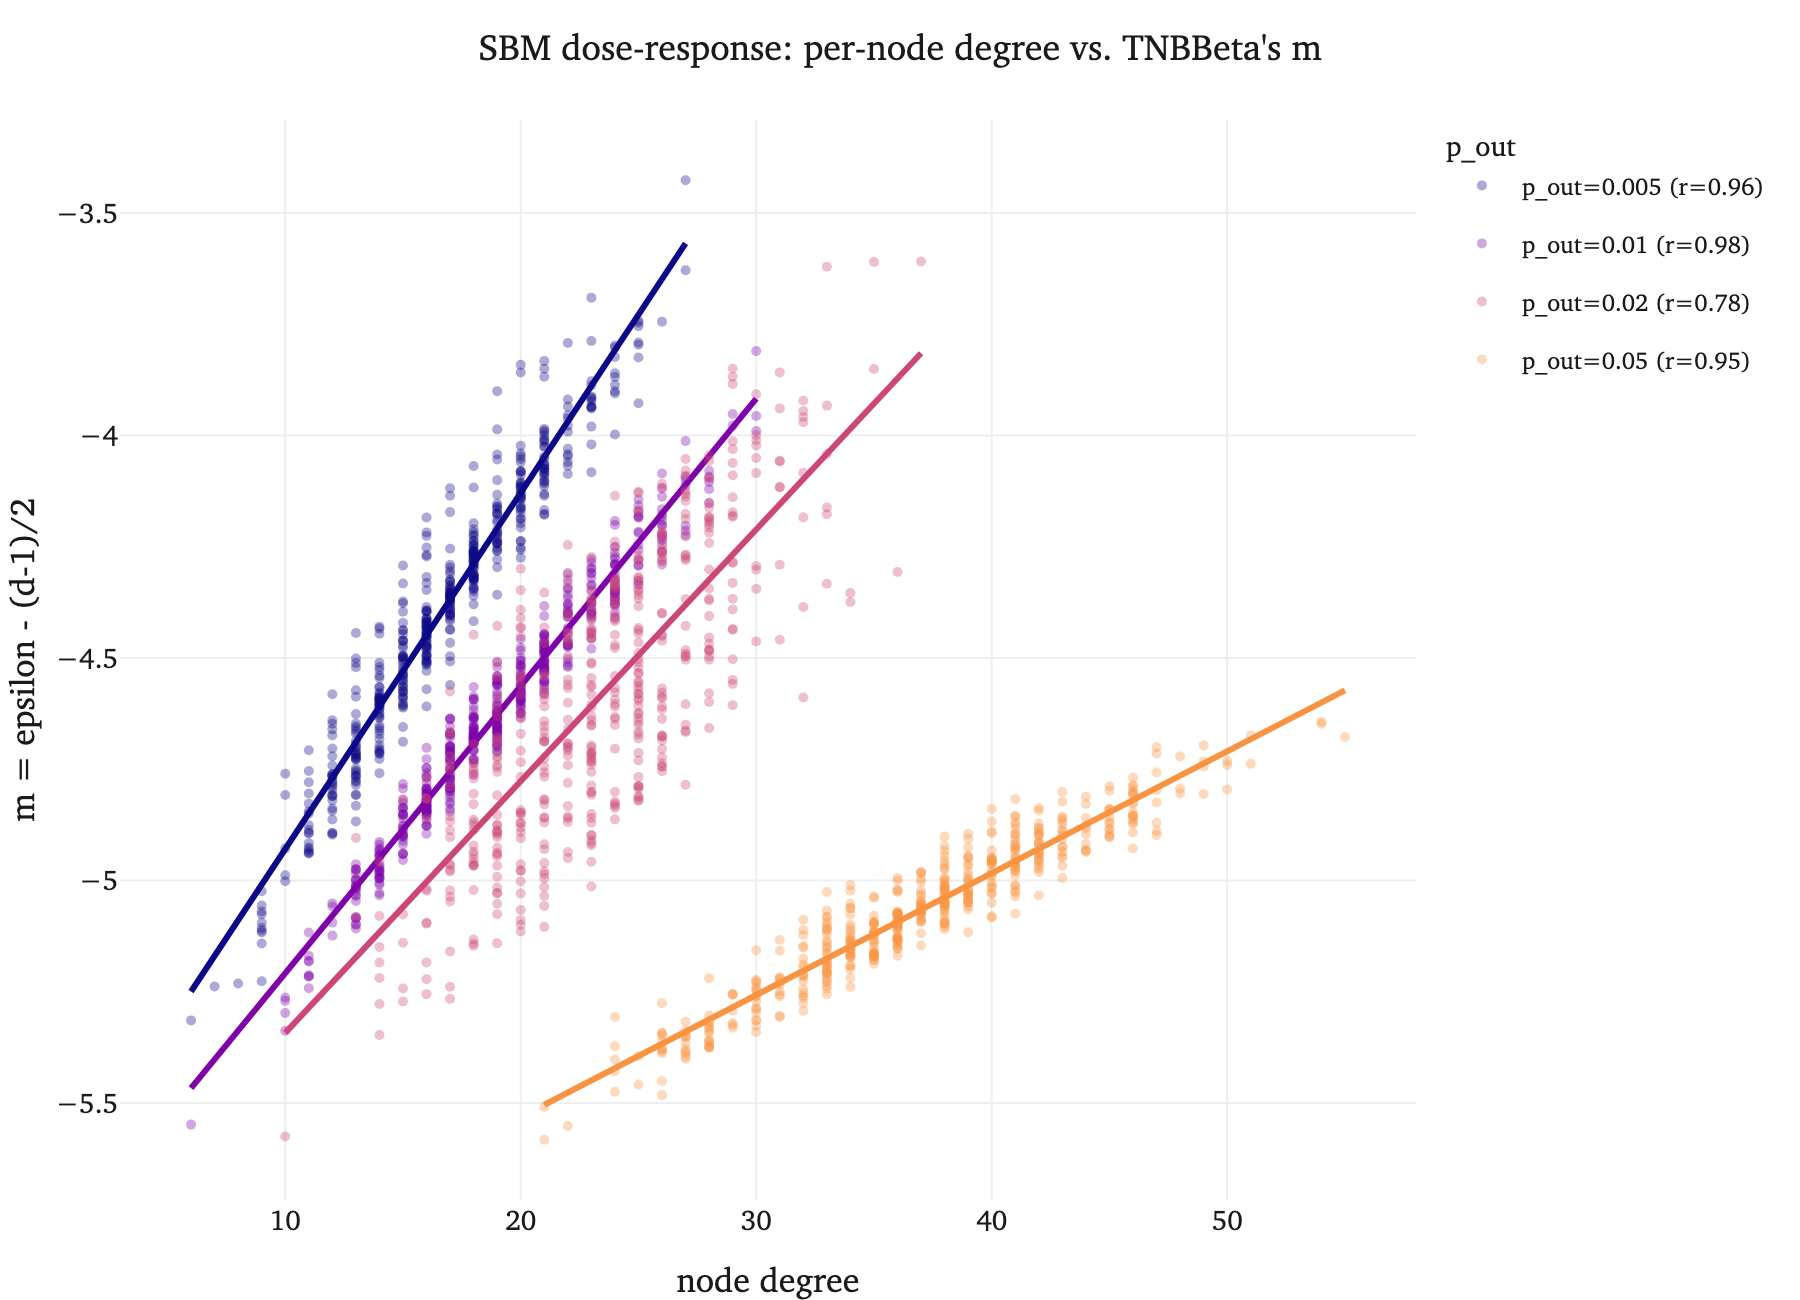
\includegraphics[width=\textwidth * 6 / 8]{assets/sbm_degree_vs_m.png}
    \caption{Per-node degree vs.\ $m$ on the synthetic graphs, one color per $p_{\text{out}}$ level, with
    a line of best fit and Pearson $r$ per level.}
    \label{fig:sbm-degree-vs-m}
\end{figure}
We find that, on average, as $p_{\text{out}}$ increases, $m$ becomes \textit{more} negative. Namely, multimodality
correlates with how densely-connected the graph's \textit{communities} are. What is more interesting, and yet to be explored,
is that $m$ and $\text{deg}(i)$ are \textit{positively} correlated\footnote{We omit the results for $p = 0.1$ as those produced a constant value of $m$. This is yet to be investigated.}. One would expect that nodes with high degree and thus a higher
chance of links to several other communities take greater advantage of multimodality. The above, in fact, shows the opposite.